\newpage
\section{Searching}
\subsection{Unbound Searching}
give a sorted list and the function
\begin{align*}
    F(i)=\left\{ \begin{array}{ll}
        0 & \text{ if }0<i<n\\
        1 & \text{ if }i\ge n
    \end{array} \right.
\end{align*}
Only we can do is to query $F(k)$. How to find $n$?

可以使用二分, 但我们不知道最大的边界在哪.

Let $S_A(n)=m$ if algorithm $A$ uses $m$ queries to find $n$. 

\subsubsection{Preliminary Algorithms}
\begin{itemize}
    \item Unary search $B_0$
    \item Binary search $B_1$
\end{itemize}

\begin{figure}[H]
    \centering
    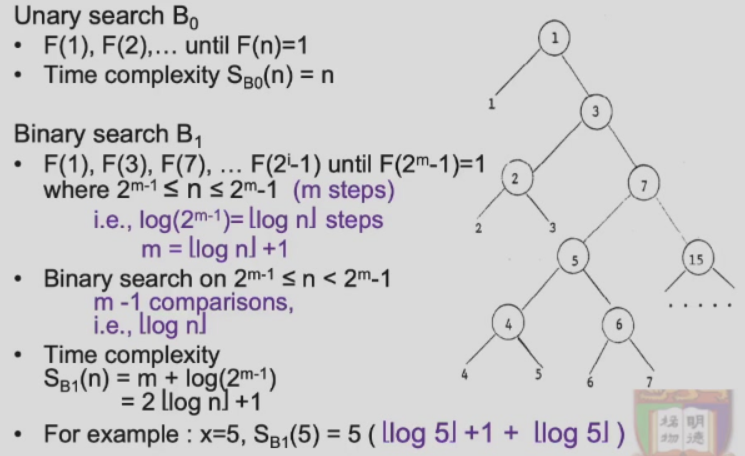
\includegraphics[width=0.309\textwidth]{pic/DAA4/Preliminary Algorithms}
    \caption{Preliminary Algorithms}
\end{figure}


\subsubsection{Higher Binary Search}
\begin{itemize}
    \item Double binary search $B_2$
    \item Triple binary search $B_3$
    \item $k$ binary search $B_k$
\end{itemize}

\begin{figure}[H]
    \centering
    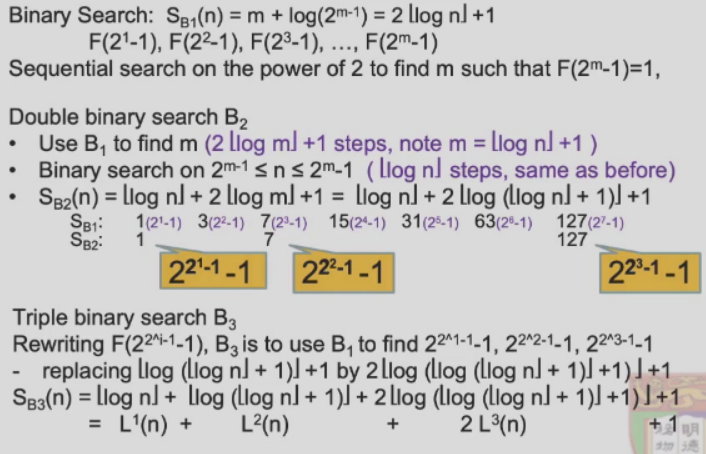
\includegraphics[width=0.309\textwidth]{pic/DAA4/Higher Binary Search}
    \caption{Higher Binary Search}
\end{figure}


\subsubsection{Ultimate Algorithm}
determine $k$ for $B_k$ to find $n$.

\begin{figure}[H]
    \centering
    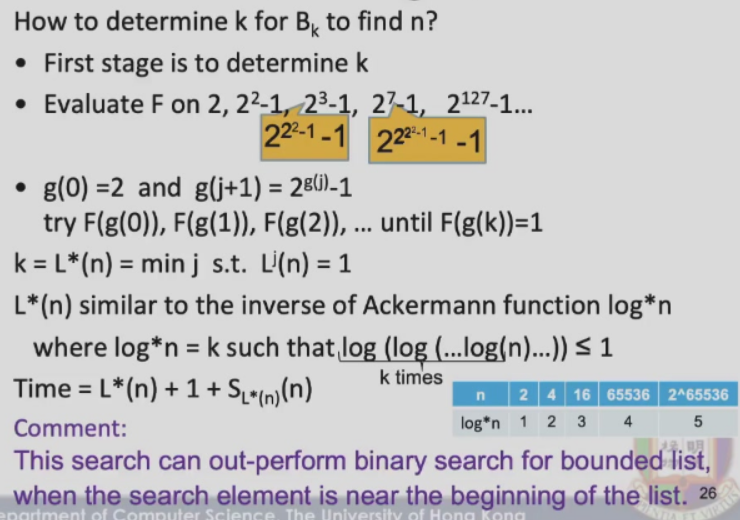
\includegraphics[width=0.309\textwidth]{pic/DAA4/Ultimate Algorithm}
    \caption{Ultimate Algorithm}
\end{figure}


\subsubsection{Sketch of Lower Bound}
\begin{figure}[H]
    \centering
    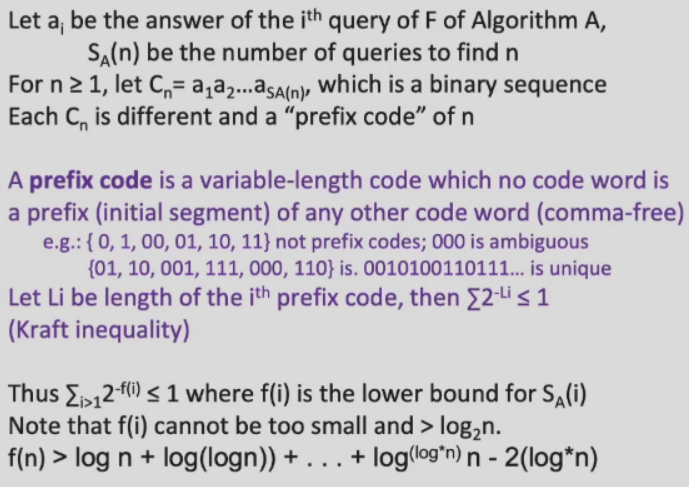
\includegraphics[width=0.309\textwidth]{pic/DAA4/Sketch of Lower Bound}
    \caption{Sketch of Lower Bound}
\end{figure}

\subsection{Find X in a Sotred Matrix}
\begin{figure}[H]
    \centering
    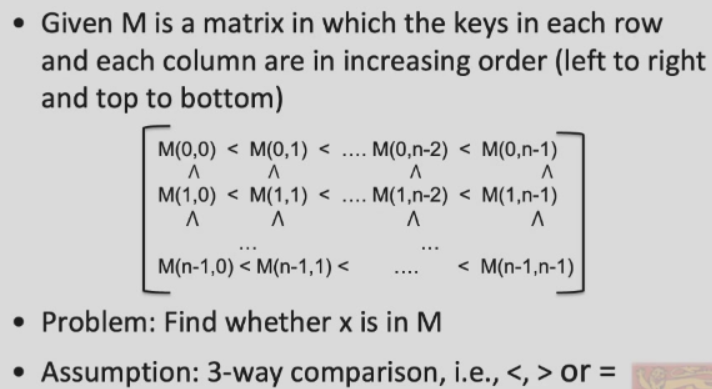
\includegraphics[width=0.309\textwidth]{pic/DAA4/Find X in a Sotred Matrix}
    \caption{Find X in a Sotred Matrix}
\end{figure}

\subsubsection{Solution}
\begin{figure}[H]
    \centering
    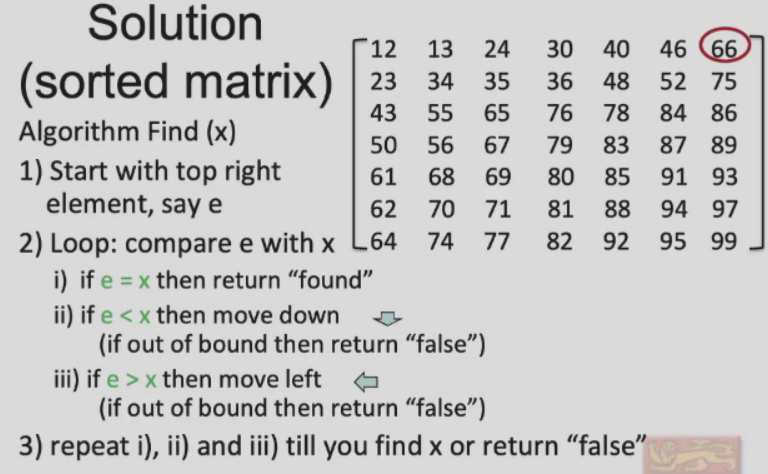
\includegraphics[width=0.309\textwidth]{pic/DAA4/Solution}
    \caption{Solution}
\end{figure}
Complexity: $2n-1$ comparisons

\subsubsection{Lower Bound}
\begin{figure}[H]
    \centering
    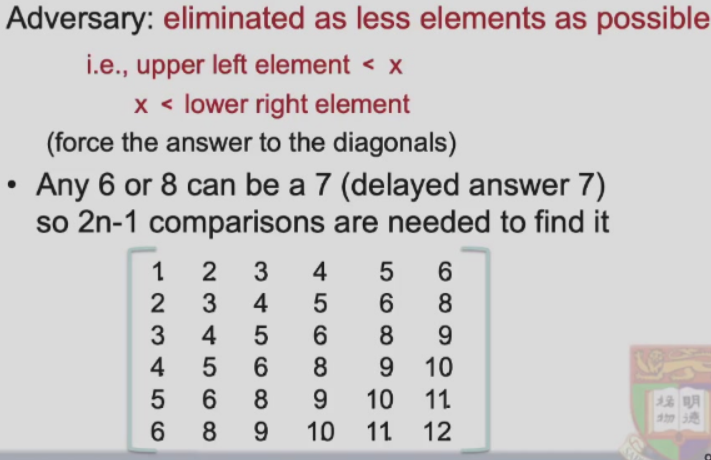
\includegraphics[width=0.309\textwidth]{pic/DAA4/Adversary}
    \caption{Adversary}
\end{figure}


